\chapter{Implementation}

 
\section{Benchmarking, Studies and Researches}
Before starting writing code, we did a study on existing metaverses platforms and we picked a bunch of blockchains to pick one for our project. The number of networks is getting in increase but the majority uses one of this 4 blockchains: Ethereum, Polygon, Solana and Cardano.

\subsection{Ethereum}
Ethereum is a decentralized platform that runs smart contracts: applications that run exactly as programmed without any possibility of fraud or third party interference. It is the most widely used blockchain for writing smart contracts. Examples of metaverse platforms based on Ethereum are \textit{Decentraland}, \textit{Cryptovoxels}, and \textit{The Sandbox}

\subsection{Polygon}
Polygon is a layer 2 solution that uses Ethereum’s smart contracts as its foundation. It scales Ethereum’s transactions by using a network of sidechains. It supports metaverse platforms such as \textit{Bloktopia}: a
decentralized VR experience that allows users to study, earn,
play, and purchase land in a unique 21-story spatial structure

\subsection{Solana}
Solana is a high-performance blockchain that can process up to 50,000 transactions per second. It uses a Proof of History consensus algorithm which allows it to achieve these high speeds without sacrificing security. It was developed to power the next generation of
metaverse platforms and powers \textit{the Star Atlas metaverse}.

\subsection{Cardano}
Cardano is a decentralized public blockchain and cryptocurrency project and is fully open source. Cardano is developing a smart contract platform which seeks to deliver more advanced features than any protocol previously developed. It is the first blockchain platform to evolve out of a scientific philosophy and a research-first driven approach. The development team consists of a global collective of expert engineers and researchers. Cardano powers \textit{the Pavia} metaverse platform.
\bigskip

To get more specific regarding what each network is capable of doing, We provide as follows, a table differentiating each technical detail between them:


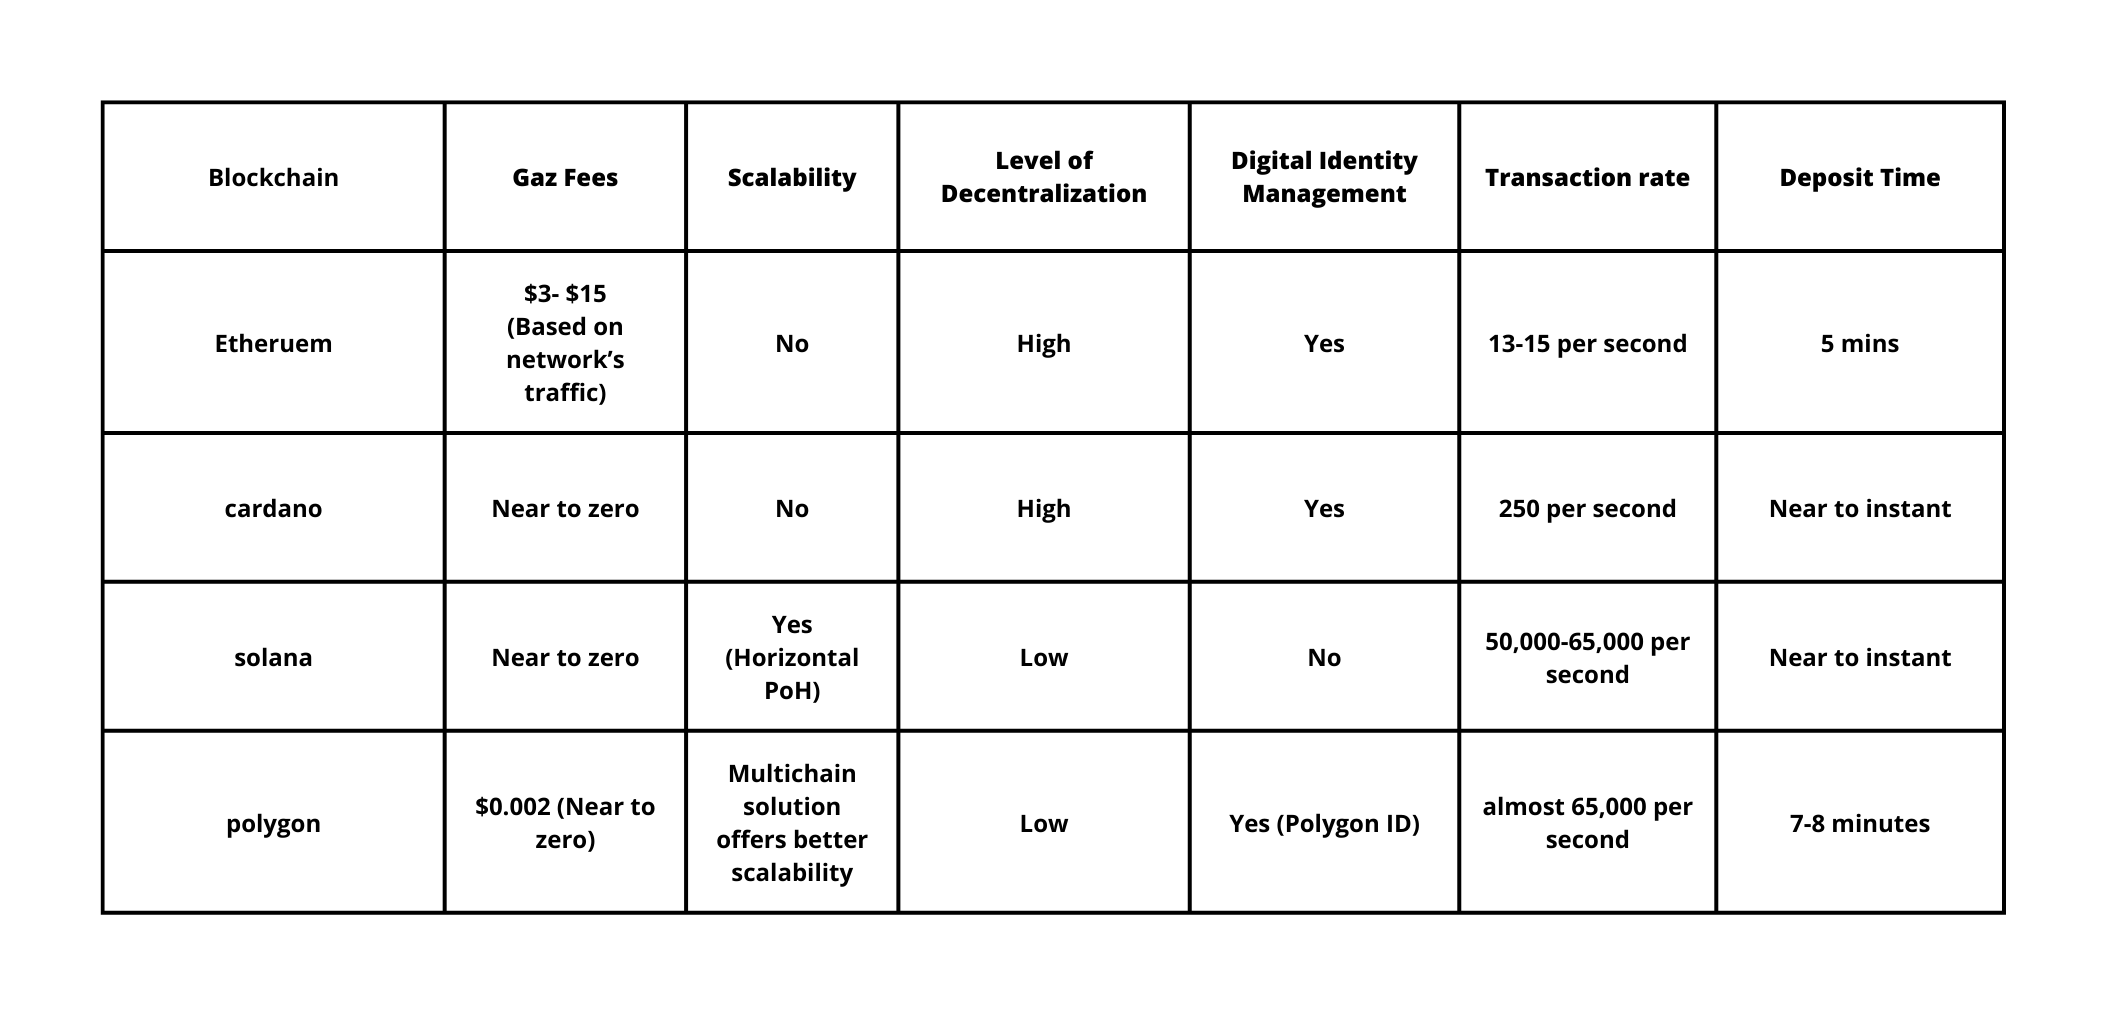
\includegraphics[width=1\textwidth, inner]{assets/comparaison.png}

As we can see, Polygon and Solana are much faster and cheaper than Ethereum, which is \textbf{very} important, since every action in the blockchain is going to be executed with fees that's the users will pay, it should be close to zero else we won't be able to attract them into the platform. Plus since a lot would join, we should consider the scalability of the infrastructure where Ethereum is not a safe option in this case. Moreover, The developer experience matters, Solana uses The Rust programming language to write smart contracts wheres the others use Solidity, and Rust is known to be an extremely complexe programming language so for faster development Solidity is a much friendly programming language to develop with. 
\bigskip
After careful considerations, we decided to pick Polygon as our Metaverse decentralized network. 

\section{Why Polygon}
\subsection{Gaz Prices}
Polygon has very cheap Gaz prices compared to other blockchains like Ethereum.

\subsection{Transactions' Rate}
About 65,000 transactions are beeing mined every second.

\subsection{EVM Compatible Blockchain}
Polygon runs on the Ethereum Virtual Machine using Solidity which is very developer friendly. In fact, its' learning curve is exponential.

\subsection{Compatible with Top NFT Marketplaces}
Polygon, alongside with Solana, Etherium are supported by OpenSea, the biggest NFT marketplace in the world. Rarible, and a tons of others, also support it.

\subsection{Code base compatibility}
We can very easily migrate the whole project to any other EVM based blockchain in the future, and this is very important since Ethereum 2.0 is around the corner.
 
 \section{Technology Stack}
\subsection{Solidity}
Solidity is a contract-oriented, high-level language for implementing smart contracts. It was influenced by C++, Python and JavaScript and is designed to target the Ethereum Virtual Machine (EVM). it is statically typed, supports inheritance, libraries and complex user-defined types among other features. Once deployed, a smart contract can be interacted with by any Ethereum user.

\subsection{Hardhat}
A hardhat is a Ethereum development tool that allows you to test Ethereum smart contracts and Dapps on a private Ethereum network. Hardhat comes with a built-in task runner and a plugin system that makes it easy to develop, test, and deploy Ethereum projects.

\subsection{Typescript}
Typescript is a popular programming language that is often used in conjunction with hardhat ethereum. It is the main language for deploying, and testing the smart contracts with Unity Tests.

\subsection{Infura}
Infura is a service that provides access to the Ethereum blockchain. It is used by dapps to connect to the Ethereum network without having to run a full Ethereum node. We have used it to get access to Rinkeby Network, Polygon Mumbai Network, and IPFS (Decentralized Storage).

\subsection{React}
React is a JavaScript library for building user interfaces. Its purpose in this context is to create websites to demo the use of the blockchain contracts in a form of a proof of concept.
 




\section{The Decentralized Identity}

\section{The Tickets Marketplace}

\section{DAO | Decentralized Autonomous Organization}